\chapter{Firewalls}
\label{ch:firewall}
A \textbf{firewall} is a device, either hardware or software, located between two areas of a network with different levels of trust. It is not only something between one network and the Internet, and it is a fundamental component in the security of a network, especially in IPv6 networks (because of autoconfiguration).

Firewalls have a simple interface specifying which kind of traffic can or cannot pass through them. They are a single point of failure, because every single packet of traffic has to pass through them, and thus if anyone bypasses it, then it is rendered useless. For this reason it is mandatory that a firewall be super-resistant to anything, meaning that it must be redundant and totally trusted; configuring one is difficult and should never be done by non-experts.

The most simple firewalls separate a local area network (high trust level) from the Internet (minimum trust level). We could also have, however, two areas of the same network, like an administrative area and a technical area, which have a firewall between them. Generally speaking, we could need more firewalls than we might think.

\begin{figure}[h]
    \centering
    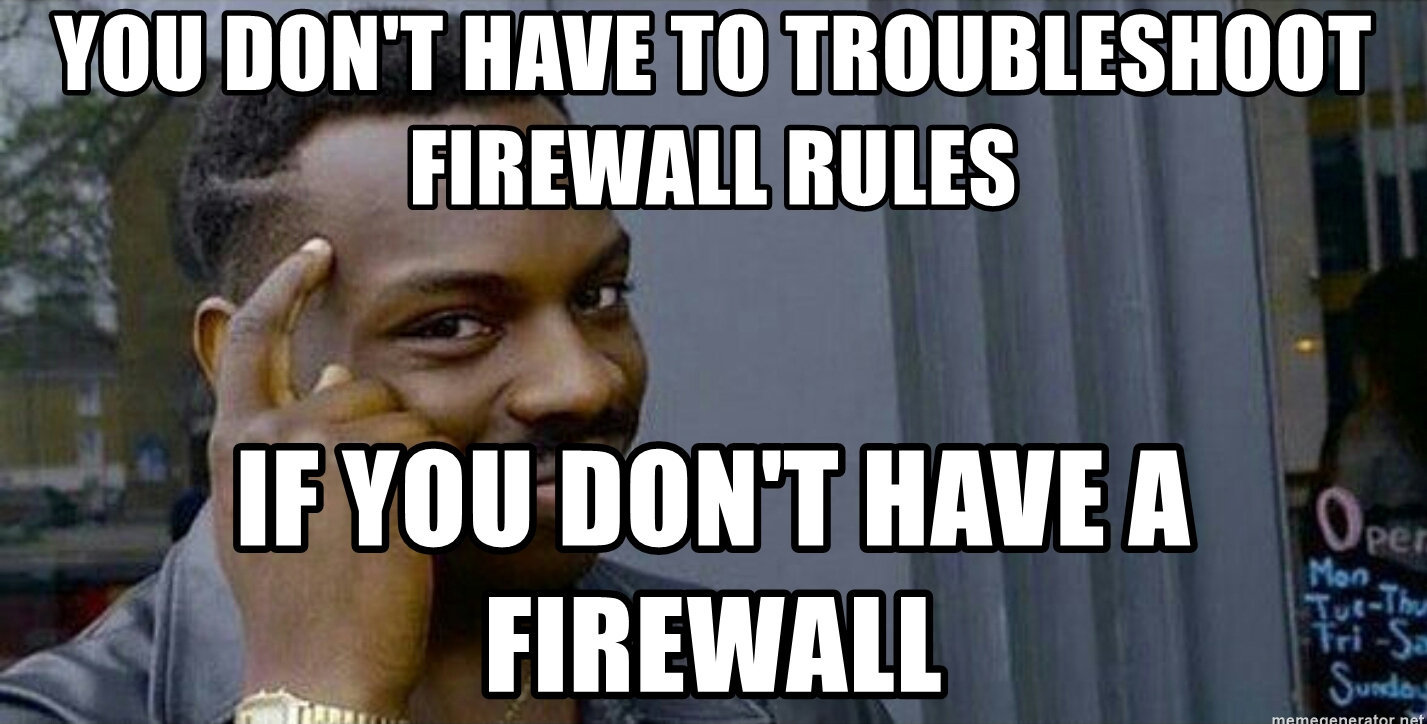
\includegraphics[scale=0.3]{img/fw_rules_meme.jpg}
    \decoRule
    \caption{Having no firewall at all is an option, too.}
    \label{fig:fw_rules_meme}
\end{figure}

%----------------------------------------------------------------------------------------

\section{Types of firewalls}
There are three kinds of firewalls:

\begin{itemize}
    \item \textbf{packet filter firewall}: the simplest firewall, it inspects each packet, and decides according to some rules if it can pass or not (it is a memoryless machine; totally garbage);
    \item \textbf{stateful firewall}: extremely more complicated, as it is a stateful machine (it has memory), it can decide if a packet can pass or not according to what happened in the past at layers 3 and 4 (IP and TCP; the only firewall acceptable for use);
    \item \textbf{application layer firewall}: an even more complex machine, it checks packets up to layer 7, meaning that it goes up to the point of inspecting the application level data that is being transmitted (it violates privacy by design, should not be used).
\end{itemize}

In order to work, application level firewalls must know the application layer protocol that is being used, hence they have to understand not only public/standard protocols, but also proprietary protocols (since they have to decode them and inspect the data). When a new protocol is created, or when any other protocol is changed even slightly, application level firewalls must be updated, otherwise they become obsolete. This fact creates a noticeable problem, because the update is not trivial, and the more complex the system, the more are the chances that it will introduce bugs (vulnerabilities) in the system - and guess which is the one component of a system that should never have vulnerabilities? Yep.

Application level firewalls are dramatically effective, but they are an example of a case in which we must decide whether the cure is worse than the disease: the worst thing that an attacker can do by hacking a stateful firewall is to let some traffic pass (that was not supposed to pass), while hacking an application level firewall would allow him/her to inspect every single bit that passes through that point, effectively making it a man in the middle.

%-------------------------------------------

\subsection*{Hardware vs. software firewalls}
Firewalls can be either hardware of software. Hardware firewalls consist of a FPG\footnote{A field-programmable gate array (FPGA or just FPG) is an integrated circuit designed to be configured by a customer or a designer after manufacturing – hence the term "field-programmable".} or some other kind of micro controller, while software firewalls - the most common ones - consist of a piece of software running on top of an operating system on a small device, like a Raspberry Pi or an Arduino. Note that even though hardware firewalls do not have an underlying OS, they still implement some software, but in the form of only one application forever looping on the chip.

The main difference between hardware and software firewalls is that the latter have to also make sure that the OS and its related processes are bug-free. The most important thing is then to avoid mixing functionalities: the firewall machine should only run the firewall itself, while all other services (like web servers) should be executed on another device, otherwise whoever attacks other processes will end up compromising the firewall, too.

%----------------------------------------------------------------------------------------

\section{Firewall placement}
By now, it should be clear that we \textit{need} a firewall. Everybody has a firewall in their router, although almost nobody configures it correctly\footnote{Neither did you. Do it. Now.}. But where should a firewall be placed?

Like mentioned before, in any network there are at least two security areas:

\begin{itemize}
    \item the \textbf{internal area}: an internal network containing all user devices, internal servers and databases (basically the part that needs to be most protected);
    \item the \textbf{demilitarized zone} (\textbf{DMZ}): this is the area which contains web, e-mail and DNS servers, together with all the other services which require to be directly accessible from the outside.
\end{itemize}

\begin{figure}[h]
    \centering
    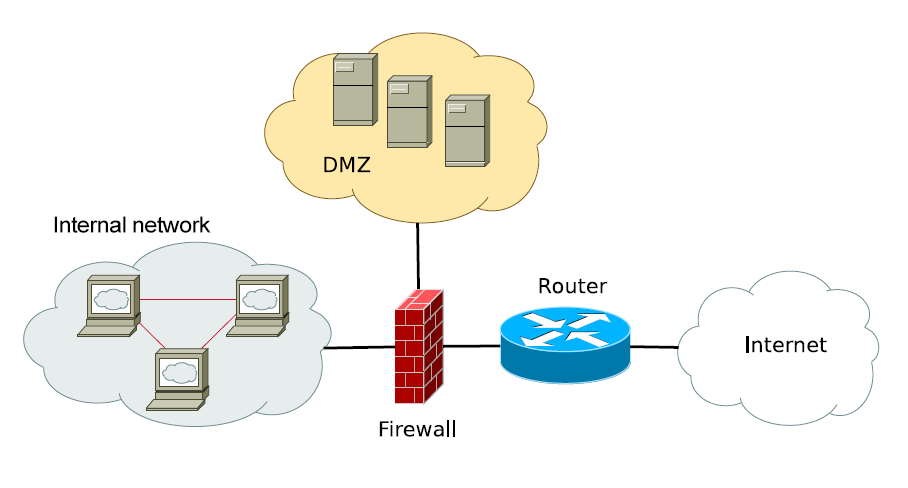
\includegraphics[scale=0.7]{img/fw_placement.png}
    \decoRule
    \caption{A simple scheme showing the position of the firewall in a network.}
    \label{fig:fw_placement}
\end{figure}

DMZ services can be accessed from both the internal area and the outside (the Internet); while the same services can go outside in turn, they are \textit{forbidden} to reach directly the internal network.

The demilitarized zone is \textbf{expendable}: it is where we place services that must be reached from the Internet, but it is no big deal if they are compromised (we will just reinstate them without crying, at least not too much). This is also the place where countermeasures are important, because it can be attacked since we allow traffic from the Internet to flow here directly. The internal network, vice versa, has different security requirements.

Is one firewall enough? Yes; it has three interfaces, which should be as much separated as possible, even physically (using different Ethernet connections - note that they cannot share the same switch).

If we have enough money, we can install \textbf{two firewalls}; their configuration would be basically the same (see figure \ref{fig:two_fws}), but they would only have two interfaces each. However, the rules would be far more complicated, because they would have to be enforced by both firewalls. The purpose of having two firewalls is that if an attacker bypasses the first one, it should then have to bypass the other, too, resulting in a longer and more complicated attack. Of course, this strategy is only valid if the two firewalls are completely different (in type, brand, operating system\footnote{Different operating system have different firewalls because of their completely different codebases. This is a useful feature because even if one firewall has a vulnerability (people are human, and humans err), in the other one the same vulnerability probably does not exist because they do not share the codebase, and this means that the configurations of the two firewalls will be completely different in terms of logic.} and hardware).

\begin{figure}[h]
    \centering
    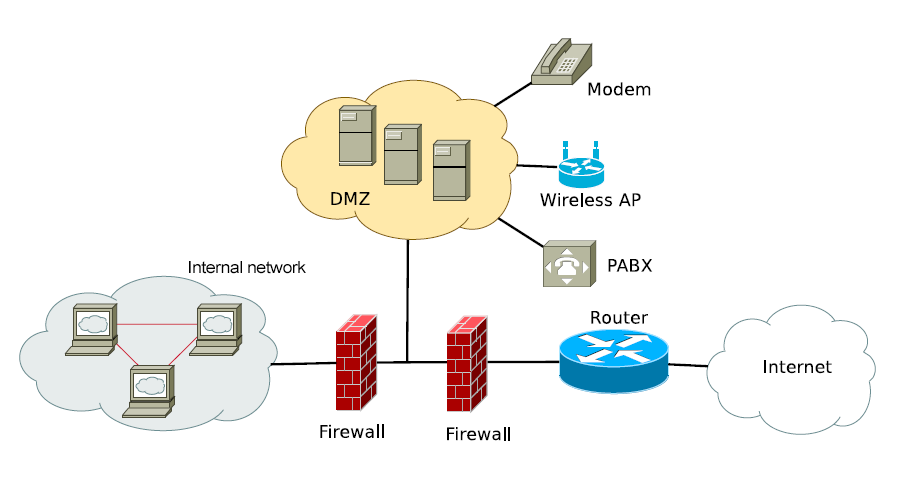
\includegraphics[scale=0.7]{img/two_fws.png}
    \decoRule
    \caption{Two-firewall configuration. If we put a NAT between the two firewalls and the DMZ, one of the firewalls will not understand where packets are supposed to go and/or where they come from.}
    \label{fig:two_fws}
\end{figure}

This fundamental requirement, however, makes this kind of configuration a headache not only for an attacker, but also for the sysadmin, and it also multiples the probabilities of having some error in the configuration (which in in turn would lead to vulnerabilities): it is a good idea, but one that could backfire easily and very badly. For this reason, in most cases it is better to have a single firewall which we know perfectly how to configure.

%----------------------------------------------------------------------------------------

\section{Netfilter}
\textbf{Netfilter} (iptables) is a framework provided by the Linux kernel that allows various networking-related operations to be implemented; in particular, it offers various functions and operations for packet filtering, network address translation and port translation, which provide the functionality required for directing packets through a network and prohibiting packets from reaching sensitive locations within a network. Netfilter is the Linux firewall\footnote{It is not related to MacOS, which uses PacketFilter instead.} and, being very accessible, it represents an interesting case study for a number of reasons.

Note that when accessing the Linux firewall, we actually access two pieces of software: one is iptables, a user-space program that allows a system administrator to configure the IP packet filter rules (basically the interface that we can see on the screen), while the other is the actual kernel-space\footnote{The user-space can \textbf{abstract from hardware}, while the kernel-space cannot (although some kernel modules can abstract, too). Writing kernel-space code is a nightmare (fig. \ref{fig:meme_this_is_fine_fw}): even the slightest mistake will lead to a BSOD, because the kernel has unprotected access to the hardware and memory, and is incredibly difficult to debug.} firewall.

\begin{figure}[h]
    \centering
    
\includegraphics[scale=1]{img/this_is_fine.jpg}
    \decoRule
    \caption{Writing kernel code is as simple as riding a bicycle, except that the road is on fire, the bicycle is on fire, \textit{everything} is on fire.}
    \label{fig:meme_this_is_fine_fw}
\end{figure}

%----------------------------------------------------------------------------------------

\section{Filtering}
Generally, a firewall must check every packet that passes through the network, must not have any bugs and must be the smallest, fastest piece of software in a system. iptables serves as a shield from whatever \sout{shit} bad stuff the user might do (the user should never interact directly with Netfilter). Other operating systems implement even more advanced packet filters: for example, the Cisco IOS (Internetwork Operating System) is able to perform live changes to the rules without losing packets incoming/outgoing during the changes themselves.

\vspace{0.5em}

\emph{Example} An iptables rule could be \texttt{iptables -t filter -D INPUT –dport 80 -j ACCEPT}

This rule can be interpreted as "accept all packets incoming to port 80":

\begin{itemize}
    \item \texttt{-t filter}: table;
    \item \texttt{-D input}: chain;
    \item \texttt{–dport 80}: matching rule;
    \item \texttt{-j ACCEPT}: target.
\end{itemize}

\vspace{0.5em}

\emph{Example} Let us examine the example configuration in figure \ref{fig:fw_example}. A firewall can be seen as a host with at least two network interfaces (1 and 2), connecting two networks (A and B); packets arrive to one of the NICs, are filtered and then forwarded towards the other NIC. Suppose, for simplicity, that packets can only flow from network A to network B.

\begin{figure}[h]
    \centering
    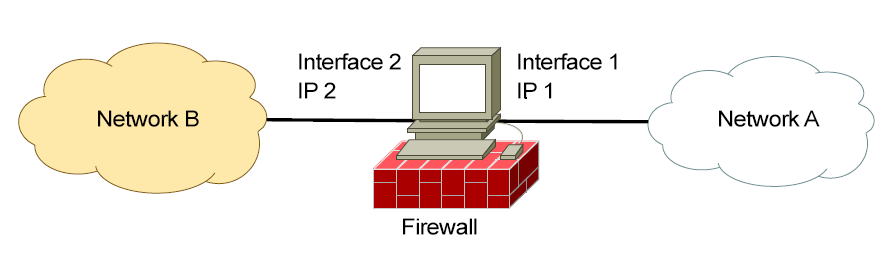
\includegraphics[scale=0.7]{img/fw_example.png}
    \decoRule
    \caption{An example firewall configuration.}
    \label{fig:fw_example}
\end{figure}

\begin{figure}[h]
    \centering
    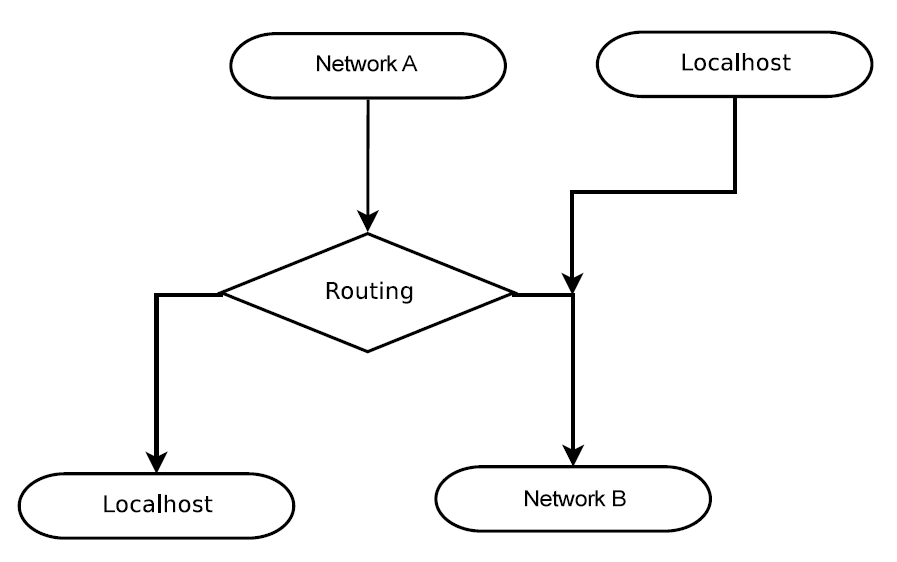
\includegraphics[scale=0.7]{img/fw_logic.png}
    \decoRule
    \caption{Flowchart diagram of the data flow in the example firewall configuration in figure \ref{fig:fw_example}.}
    \label{fig:fw_logic}
\end{figure}

If we represent this data flow with a flowchart diagram (fig. \ref{fig:fw_logic}), we can see that packets can come from either A or the localhost (the firewall), and they can go to either to B or the localhost. Since we are assuming that the localhost is not completely brainless and can send data itself (although we could object this assumption), then localhost can send data to B directly, while data from A must pass through the routing table. Allowing localhost to localhost packets to avoid passing through the routing would yield a a slightly different layout.

This configuration is relevant for the firewall, and it depends on the operating system: on Linux/BSD systems the localhost is, from the point of view of the kernel, a TCP socket, but actually it consists of a virtual interface called \textbf{loh} (\texttt{localhost}/\texttt{127.0.0.1}). If we open a socket in localhost B and want to send data through it to localhost A, it will not pass through the routing point (the piece of software that actually checks the routing tables), because the kernel knows who is sending it.

%-------------------------------------------

\subsection{Chains and tables}
On a high-level, iptables usually contains multiple \textbf{tables}; tables contain multiple \textbf{chains}, which can be built-in or user-defined, and chains contain multiple rules, which in turn are defined for the packets. Chains identify the point in the kernel where the filtering is done, while tables associate a function to each rule. Different firewalls have different tables and different chains, even though the general organization in tables is almost always the same because it is logical.
We can do many different things in the chains, like \textbf{accepting} or \textbf{dropping packages}, modifying them (\textbf{mangling}) and \textbf{logging messages}.

Netfilter chains are organized as shown in figure \ref{fig:netfilter_chains}, and are named with predefined titles:

\begin{itemize}
    \item \textbf{prerouting}: a sort of pre-check, this is where every packet is inspected before checking where it will go;
    \item \textbf{postrouting}: redundant, as routing would work just fine without this step;
    \item \textbf{output}: the equivalent of \textit{prerouting} for packages coming from a local socket;
    \item \textbf{input}: this is where packets incoming to the local host are analyzed;
    \item \textbf{forward}: the same as \textit{input}, but for packets directed towards the Internet.
\end{itemize}

\begin{figure}[h]
    \centering
    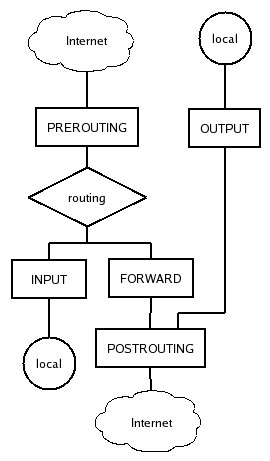
\includegraphics[scale=1]{img/netfilter_chains.png}
    \decoRule
    \caption{Filter table chains.}
    \label{fig:netfilter_chains}
\end{figure}

We are, however, missing something: the diagram in fig. \ref{fig:netfilter_chains} shows not how a firewall works, but how \textit{any} program that sends data works: if we write our own piece of code, packets from our computer to our Internet ports do not go through the router. This is true but also false, in the sense that the routing in figure \ref{fig:netfilter_chains} is responsible for forwarding packets from one port to another. The one thing that is not represented here is another piece of software that decides which output port must be used for a certain socket (port decision).

In order to easily distinguish between groups of similar data inspection flows, iptables has four built-in tables which group together rules that have the same function: the \textbf{filter table}, \textbf{NAT table}, \textbf{mangle table} and \textbf{raw table}. Each table contains chains of rules that can also be called by other tables.

\begin{figure}[h]
    \centering
    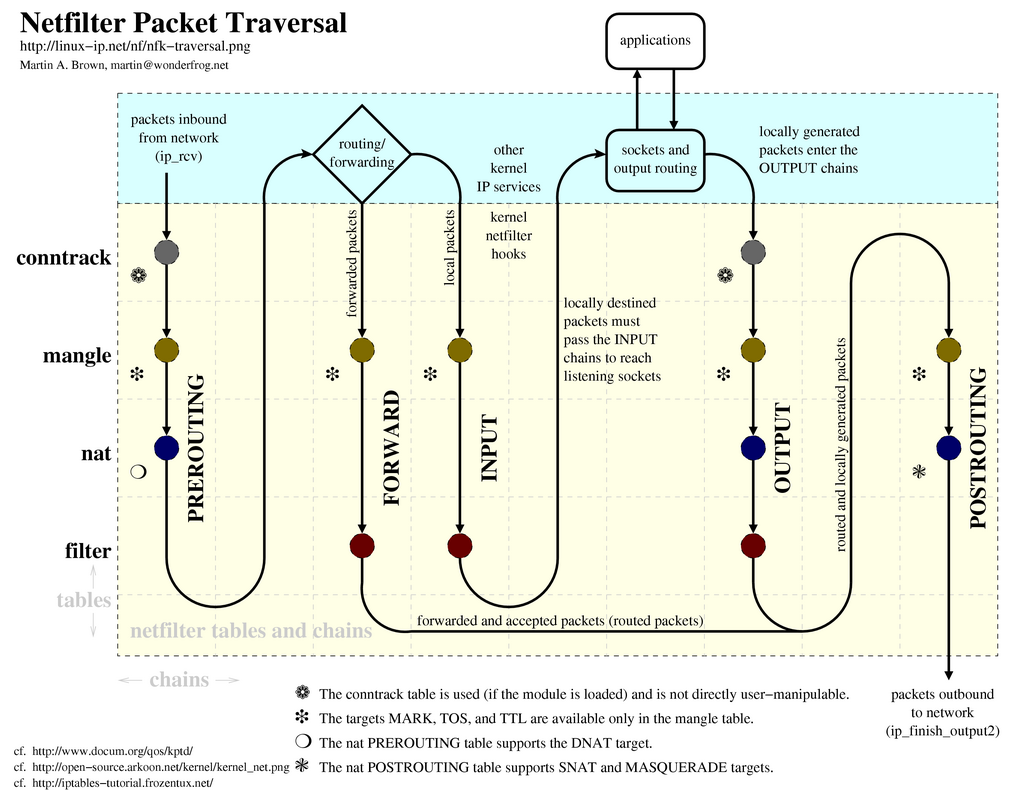
\includegraphics[scale=0.6]{img/netfilter_packet_traversal.png}
    \decoRule
    \caption{Netfilter packet traversal diagram.}
    \label{fig:netfilter_packet_traversal}
\end{figure}

%----------------------

\subsubsection{Filter table}

\textit{\textbf{Filter}} is default table for iptables: if we do not define our own table, we will be using this one, which is for general-purpose filtering (firewalling).

This table has the following possible targets:

\begin{itemize}
    \item \textbf{drop}: the packet is dropped without notifying the sender;
    \item \textbf{reject}: the packet is dropped and the sender is notified;
    \item \textbf{accept}: the packet continues its journey towards the destination;
    \item \textbf{log}: the packet generates a log.
\end{itemize}

A number or attacks can be performed using rejection, so we should never use it if possible. Logging should be avoided, too, because it could easily fill up the hard disk.

%----------------------

\subsubsection{NAT table}
This is where we ask ourselves why would a firewall modify packets like a NAT does. The answer is that everything that the NAT does partially applies to the firewall, too (they share the packet tracking feature, for example).

The possible targets of the NAT table are:

\begin{itemize}
    \item \textbf{DNAT} (Destination Address Translation): alters packets \textit{before} routing, in order to translate the destination IP address of the packets to something that matches the routing on the local server (commonly used by frontier firewalls to redistribute traffic on a network with multiple servers);
    \item \textbf{SNAT} (Source Address Translation): alters packets \textit{after} routing, in order  to translate packets when they are leaving the system.
\end{itemize}

In other words, DNAT and SNAT are used to make it look like a given machine (for example a webserver) can be found at a certain location, even though it is actually inside a local network behind a NAT.

%----------------------

\subsubsection{Mangle table}
This table is used for specialized packet alteration, to be done after conntrack (see below, section \ref{sec:conntrack}) (but still before any other table). It enables additional modifications, such as NAT or further filtering.

%----------------------

\subsubsection{Raw table}
iptables’s raw table is for configuration exceptions. It can be used to filter packets before they reach more memory-demanding operations such as conntrack.

%-------------------------------------------

\subsection{Conntrack}
\label{sec:conntrack}
Netfilter/iptables is a \textbf{stateful} machine, so it needs to keep track of all logical network connections or sessions, and thereby relate all of the packets which may make up that connection.

\textbf{Conntrack} is a feature that attaches a tag to every packet, in a field that can be read by everyone else, so that subsequent phases in the routing process can always know what the conntrack was thinking about a certain packet. Basically, the conntrack individuates:

\begin{itemize}
    \item fragments belonging to the same IP packet (IPv4 only, as in IPv6 this is not needed);
    \item packets belonging to the same connection;
    \item packets loosely related to each other (belonging to distinct but related connections, like in FTP\footnote{FTP, File transfer Protocol, is a remnant of the past. It has two flows, and it was useful because they could be used in multiple ways (e.g. for data transfer); however, it had the command initiated by the client, and the data flow by the server: this was neat until the NAT came, which blocked any flow starting from the server to the client. This was a problem for the firewall, too, so in order to solve it FTP would open ports which were not checked by the firewall: a very bad idea.}).
\end{itemize}

For some protocols, firewalls can inspect also application layer data and identify packets belonging to the same connection even if they do not share the same ports, by defining four states:

\begin{itemize}
    \item \textbf{new}: the kernel is seeing the packet for the first time;
    \item \textbf{established}: the packet is similar to something already seen (the conntrack contains a statement saying so);
    \item \textbf{related}: specific case for when the data transfer connection is related to the command connection;
    \item \textbf{invalid}: error-related state for unforeseen situations (normally, packets are either established or new).
\end{itemize}

\vspace{0.5em}

\emph{Example} Consider Cisco Webex Meetings, a proprietary video conferencing application: it probably has a flow of data represented by the video and audio stream and, for example, another one for the slides. The first flow would be established, while the others would be related if they go to different TCP ports.

\vspace{0.5em}
	
These states are handled by the conntrack, and are available both to the NAT and the filter table. They are interesting because they give us the ability to have a stateful firewall, since the rules into the filters are stateless (except for the fact that we can inspect the state - which is handled by the conntrack). If we have a new protocol, we can always modify the conntrack in order to understand it and to attach the proper labels to packets.

\vspace{0.5em}

\emph{Example} Generally, a firewall does not really block packets, because that would mean that someone from the inside would send packets outside that would remain without an answer. A firewall actually blocks \textit{flows} that begin from the outside.

%----------------------------------------------------------------------------------------

\section{Fault tolerance and load balancing}
\textbf{Fault tolerance and load balancing} in firewalls is an extremely important topic, because if the firewall goes down we are disconnected from the network in the best case, connected and completely unprotected in the worst.

A firewall is naturally an input/output point in a network, and if not properly managed can easily become a \textbf{bottleneck}. For this reason, and especially in high traffic networks, dividing the load between two or more firewalls is fundamental for better performance and backup solutions, so that the system is fault tolerant and resistant to any network condition.

\vspace{0.5em}

\emph{Example} In a gigabit Ethernet network the firewall must be ready to process one gigabit of data per second - which is a lot.

\vspace{0.5em}

%-------------------------------------------

\subsection{Primary backup configuration}
The fault tolerance problem can be rather easily solved by using a \textbf{backup firewall}, thus installing two firewalls instead of one (figure \ref{fig:primary_backup_fw}); note that the load balancing problem is not addressed here.

\begin{figure}[h]
    \centering
    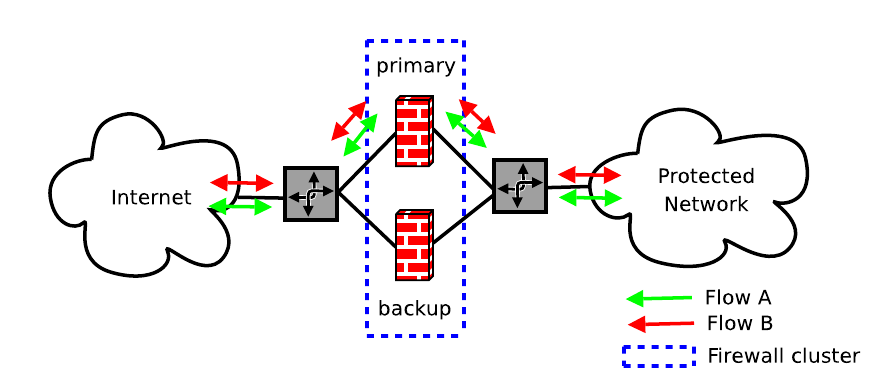
\includegraphics[scale=0.7]{img/primary_backup_fw.png}
    \decoRule
    \caption{Primary backup firewall configuration.}
    \label{fig:primary_backup_fw}
\end{figure}

There is, however, a problem associated to this solution: we cannot shut down completely the second firewall, because it must be ready to be started by an automatic configuration called the \textbf{heartbeat}. An uncommon system, the heartbeat is a very low level monitor that oversees the state of the machine and sends a beat (a positive signal) if it is working correctly; if the machine's CPU load drops to zero for some reason or is stuck at 100\% for too long (or in general, if anything goes beyond a nominal value), the heart stops the beat and the monitor understands that the device has failed, and thus wakes the second device up. Clearly, in order to work this configuration needs other devices, too: besides the firewalls and heartbeat we also have to install switches\footnote{Switches are extremely simple devices with high reliability, very difficult/unlikely to break, so they are not usually backed up like a firewall. They, too, have to be connected to the heartbeat.} to direct the traffic from the interface of the failed firewall to the second one.

This configuration is more or less efficient depending on the state of the backup firewall:

\begin{itemize}
    \item shut down (\textbf{cold swap backup}): there is no power on the CPU. If possible, the heartbeat can be programmed to put the machine up, but it would still have to boot, so it would require at least a few seconds before being operative, during which the full network would be down;
    \item sleep mode (\textbf{hot swap backup}): boot time is much lower in this case, but energy consumption is higher because the memory has to be kept active;
    \item \textbf{active}: the backup firewall is up and running, so we just have to command the switches to have it take over the traffic; energy consumption is even higher than in sleep mode.
\end{itemize}

%----------------------

\subsubsection*{Cons of the primary backup configuration}
Is the primary backup a good idea at all? Actually, not really. Reliability studies tell us that the source of problems in a computer, or most electronic devices, is not their normal operation, but the boot time: nine out of ten problems happen during boot operations.

\vspace{0.5em}

\emph{Example} A computer worked perfectly until yesterday; we shut it down, and when the following morning we boot it up, everything is broken. Sounds familiar? To me, it sure does. Check your SSD, PSU or GPU next time it happens.

\vspace{0.5em}

It is a problem of electrical nature that lies in the power source: at power on the electric spikes generated by the power block go into the computer and can fry the electronics. This is why many people say that it is safer to leave the computer in sleep mode than to shut it down completely, and for this same reason it is much better using a hot swap backup firewall configuration. So in general it is better to never shut down neither the computer or the firewall, nor to take for granted that they will power up the next time they will be needed.

Nowadays there is another problem, too: the reliability of the secondary memory. One thing is the reliability of a physical hard disk drives (HDDs), another is that of solid state drives (SSDs), which have a MTBF\footnote{MTBF, short for Mean Time Between Failures, is the predicted elapsed time between inherent failures of a mechanical or electronic system, during normal system operation.} proportional to the number of writes on the drive, so it heavily depends on their use.

The last, obvious con of having a second firewall as a backup solution is that, well, we had to pay for a second firewall that normally does nothing, more like buying a second car just to be safe and leave it into the garage: not a great idea, especially if we are on a tight budget.

%-------------------------------------------

\subsection{Multi-primary multi-path firewall cluster}
A second, better option is to let the second firewall do something. In this case we have a \textbf{low balancing} configuration, where the whole block of firewalls acts as one single firewall. This solution is better because we can have $n$ smaller firewalls that are able to globally handle the traffic from network A to network B, and if one of them fails the load balancer will handle the situation, rerouting the traffic towards the other firewalls (remember that, in general, load balancers are a bottleneck.).

At the end of the day the overall capacity of the firewall will be down of just $\frac{1}{n}$, so it is a win-win situation that yields better money and better configuration with respect to simple redundancy. The load balancer also allows us to take down a firewall for maintenance anytime, without any problems.

%-------------------------------------------

\subsection{Multi-primary hash-based stateful firewall-cluster}
The most useful configuration, this one does not involve a load balancer. Instead, every firewall has a numerical ID from $0$ to $n-1$ (for $n$ firewalls); each grey box in figure \ref{fig:multiprimary_backup_fw} evaluates an incoming connection through a tuple $T = IP_s, IP_d, port_s, port_d, protocol$. For each tuple, if $hash(T) \% 2 == ID$, then the connection is filtered, otherwise it is ignored. In this way the firewalls autonomously distribute the traffic between them. A heartbeat is needed in order to correctly manage failures.

\begin{figure}[h]
    \centering
    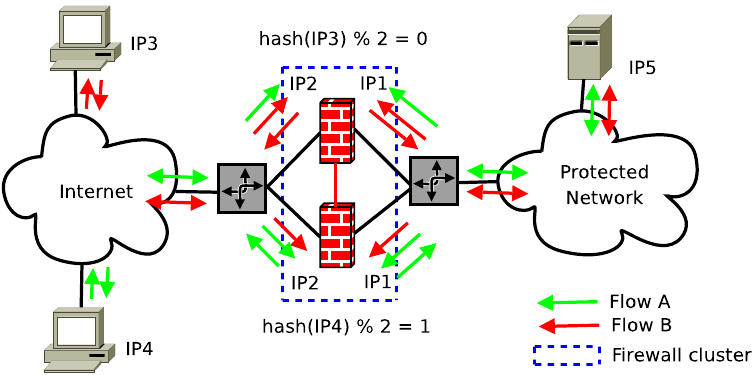
\includegraphics[scale=0.7]{img/multiprimary_backup_fw.png}
    \decoRule
    \caption{Multi-primary hash-based stateful firewall-clusters configuration. The grey boxes do not just switch from one Ethernet port to the other, but also split and balance the traffic between the machines. They are more complex than regular switches, but their reliability is still much greater than that of firewalls, because they can be made of just simple FPGs or solid state hardware ports (they do not need to be intelligent).}
    \label{fig:multiprimary_backup_fw}
\end{figure}

%----------------------

\subsubsection*{Conntrack state replication}
In this configuration, when a firewall fails, the flows on the failed firewall are lost. This happens because the conntrack is different for each firewall, so firewalls that will take over flows from the failed one will not understand them, and will probably drop their packets. It is then clear that for this configuration we do not only need a heartbeat, but also some way of keeping track of all conntracks, in case of failure.

There are two options to replicate the state of the conntrack:

\begin{enumerate}
    \item \textbf{continuously replicate conntracks};
    \item \textbf{periodically replicate conntracks};
    \item \textbf{poll-driven replication};
\end{enumerate}

All three methods involve creating a copy on HDDs or SSDs in a RAID configuration\footnote{RAID (Redundant Array of Inexpensive Disks or Redundant Array of Independent Disks), is a data storage virtualization technology that combines multiple physical disk drive components into one or more logical units for the purposes of data redundancy, performance improvement, or both.}.

Method 1 easily becomes cumbersome for a (not too) large number of firewalls, in networks with much traffic. Every firewall would have to handle the update of its own conntrack, send the changes to the others and then update its own with what it receives from the others.

Method 2, instead, sends the updates periodically (something like every 5, 10 or 60 seconds). We can decide on an administrative basis the period of time, and if we have more than two firewalls we can time the updates so as to completely avoid collisions on the side channel dedicated to them\footnote{These updates are extremely important, so it is better to execute them on a channel completely separated from the rest of the network, in a sort of high-speed secondary network connecting the firewalls between them.}. The downside is that if a firewall breaks between two updates, the changes in its conntrack that happened from the last update to the failure event are lost, and we will have a residual number of flows that will be dropped and rejected by the remaining firewall cluster.

\begin{figure}[h]
    \centering
    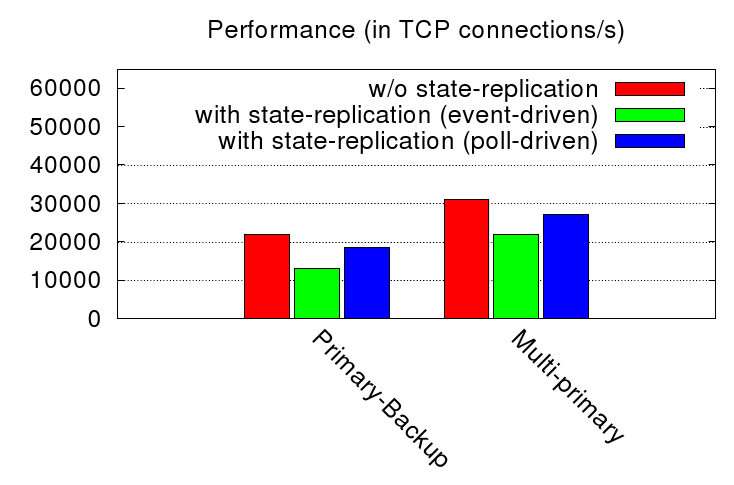
\includegraphics[scale=0.7]{img/fw_performance.png}
    \decoRule
    \caption{Comparison of firewall backup configuration performances. In terms of reliability and performance, state replication significantly impacts the overall performance of both primary backup and multi-primary configurations. Mind that this graph is slightly biased, because on one side there is a single, large firewall (primary backup), while on the other there are two (or more) smaller ones (multi-primary backup).}
    \label{fig:fw_performance}
\end{figure}

Method 3 consists of updating the conntrack state based on a poll-driven policy, instead of event-driven (like the other solutions). Its performance depends on the poll frequency, which can be as frequent as the event-driven replication or as infrequent as not having a state replication at all. The downside of this method is that even if we do not have updates, we still send data and pay the price of the poll, something that in any event-driven method would not happen.

%----------------------------------------------------------------------------------------

\section{Layer 7 filtering}
A sysadmin might want to filter layer 7 traffic for a number of reasons, like traffic log and analysis (e.g. for better configuring the whole system), traffic shaping (e.g. for flow prioritization) or protocol blocking. This kind of firewalling is necessary whenever source and destination port numbers are not sufficient to understand what kind of traffic is being analysed.

There are many different application level (layer 7) firewalls; they are extremely picky and difficult to maintain, mostly because a protocol handler must be developed inside the firewall itself, and every application (proprietary applications, too) needs a specific one.

In general, it is better to only use firewalls that do just the strictly necessary stuff (so \textit{not} layer 7 and 4 firewalls). Even if we have to block certain kinds of traffic (e.g. to prevent users from playing games or accessing social media from their offices), the best solution is to \textit{not} block them, but simply control what our users are doing, because otherwise they will most certainly deimplement our security measures.

%-------------------------------------------

\subsection{Layer 7 filtering: security}
The protocol handler in a layer 7 firewall is a critical point: there have been many cases of malware and vulnerabilities (by bad implementation) in these decoders.

\vspace{0.5em}

\emph{Example: Wireshark} A notable case was that of Wireshark\footnote{Wireshark is a free and open-source packet analyzer, used for network troubleshooting, analysis, software and communications protocol development, and education. It can tell everything about packets, even rebuild TCP and UDP flows (e.g. by looking at the traffic flow it can reconstruct the HTTP exchanges, audio files that are being sent, etc.).}, which had memory leaks in its libraries that allowed for arbitrary code execution or lead to system hangs - particularly serious issues in firewalls and similar appliances.

\vspace{0.5em}

\emph{Example: Snort RPC Preprocessing Vulnerability\footnote{Snort is an intrusion-detection system and a companion to the firewall; it is a monitor that sees if something is wrong, and it bypasses the firewall itself.}} Researchers at ISS\footnote{IBM Internet Security Systems, formerly Internet Security Systems, is a security software provider founded in 1994.} discovered a remotely exploitable buffer overflow
in the Snort stream4 preprocessor module, which allowed remote attackers to run arbitrary code on a Snort
sensor. Much like convincing a security guard -  one of our most trusted people - to do malicious things.

\vspace{0.5em}

\emph{Example: Trend Micro InterScan VirusWall Remote Overflow} An implementation flaw in a gateway allowed a remote attacker to execute code with daemon privileges (i.e. at almost administrative level).

\vspace{0.5em}

\emph{Example: Microsoft ISA Server 2000 H.323 Filter} An attacker could use a H.323 malicious malformed flow to do remote buffer overflow, basically allowing him/her to become a superuser - the worst thing that could happen in a system.

\vspace{0.5em}

\emph{Example: Cisco SIP Fixup Denial of Service (DoS)} An attacker could take the firewall down by simply sending a message.

\vspace{0.5em}

%-------------------------------------------

\subsection{Layer 7 filtering: neutrality}
A firewall must be considered only as a security policy. As network admins, our goal is the security of a system, which is driven by the risk analysis. If we find a vulnerability that can be exploited in some way, we isolate it and eventually leave the vulnerable device on the safe side of the network by putting a firewall in the middle.

No one should ever happily start blocking everything that is for some reason unwanted or unforeseen, because that is not a firewall's goal.

But, unfortunately, firewalling can also be used for bad things, i.e. enforcing rules unrelated to risk analysis, but to policies relevant to other purposes (like preventing social media access during work hours).

\vspace{0.5em}

\emph{Example} The UniFi network is limited by the GARR (Gruppo per l'Armonizzazione delle Reti della Ricerca), the Italian national computer network for universities and research. The main objective of GARR is to design and manage a very high-performance network infrastructure that delivers advanced services to the Italian academic and scientific community. This also means that every single piece of traffic on this network \textit{must} be related to university work: if we use our institutional e-mail to send a message to a family member or a friend, or to read and write Whatsapp messages, we do forbidden stuff - not for security reasons, but for administrative reasons (rules unrelated to security).

\vspace{0.5em}

We must always be mindful about which rules we implement for security reasons and which for company policies, because they are two different things, and sometimes they even collide. We have in our hands the key to \textbf{privacy}, \textbf{freedom}, \textbf{net neutrality} and \textbf{fairness} of the network.

For example, if an ISP blocks or throttles all traffic that goes towards a competitor service, that is a form of unfair business. Company-wise, if it is done because the employer does not want its employees to look at the unions' web pages, it creates a problem related to the work forces' freedom. If the same thing is done nation-wide for some (any) reason, it might lead to censorship.

Blocking a protocol is simple for a firewall, while blocking a specific site is not easy because websites have ever-changing IP addresses which firewalls cannot block. In order to prevent users from accessing specific websites, firewalls have to work at DNS level (they can block DNS requests). However, the site can just use somebody else's DNS, so even though these are measures effective against most users, they are not adequate for the most technology-oriented people. That being said, it is also true that in order to really block someone from doing anything we should prevent them for even connecting to the Internet.

\subsubsection*{Case study: the Iranian firewall}
A good (however bad for the users) example of nation-wide censorship tool is the firewall of Iran, one of the countries most strongly identified with Internet censorship.

\begin{figure}[H]
    \centering
    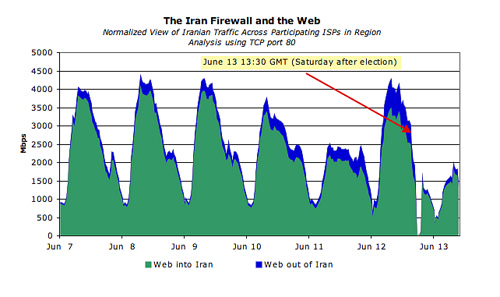
\includegraphics[scale=1]{img/l7_filtering_iran.png}
    \decoRule
    \caption{Iranian traffic during the June 2009 elections.}
    \label{fig:l7_filtering_iran}
\end{figure}

\begin{figure}[H]
    \centering
    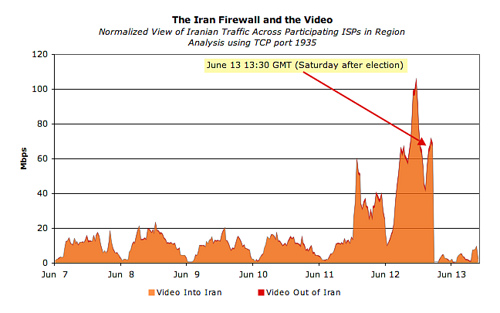
\includegraphics[scale=1]{img/l7_filtering_iran_2.png}
    \decoRule
    \caption{Iranian video-related traffic during the June 2009 elections.}
    \label{fig:l7_filtering_iran_2}
\end{figure}

It kicked in during the highly controversial 2009 Iranian presidential election, when people rioted against supposed vote manipulation and rigged elections. Not only were these riots violently suppressed by the military, but all the Internet was blocked in order to prevent people from sharing real-time news of the riots and to prevent them from internally communicating between them and organize themselves.

Note that in spite of this being an extreme case of censorship, nation-wide firewalls can be found not only, for example, in China (the Great Firewall of China), Russia ans Egypt, but also in the most unsuspecting countries. In other words, nation-wide firewalling is \textit{always} there.

\begin{figure}[H]
    \centering
    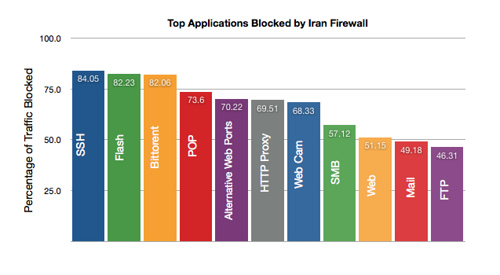
\includegraphics[scale=1]{img/l7_filtering_iran_3.png}
    \decoRule
    \caption{Top applications blocked by the Iranian firewall.}
    \label{fig:l7_filtering_iran_3}
\end{figure}

%-------------------------------------------

\subsection{Home firewalls}
Firewalls like Windows Defender are very much like face masks. During COVID-19 times, when wearing a face mask, many people go outside, see their friends, shake their hands, kiss them... they do all this because they \sout{have a face mask} are idiots. Face masks make them \textit{feel} protected, but they really are \textbf{not}. Personal firewalls are the same: they are nice and give us a sensation of protection, but it might be a very false one. Having one however is better than not, but they should not be trusted too much for the same old reason: in order to configure them we need to know exactly how to do it \textit{correctly}. Moreover, to simplify their interface, they tend to hide many options that an advanced user would find fundamental for their correct configuration.

\begin{figure}[h]
    \centering
    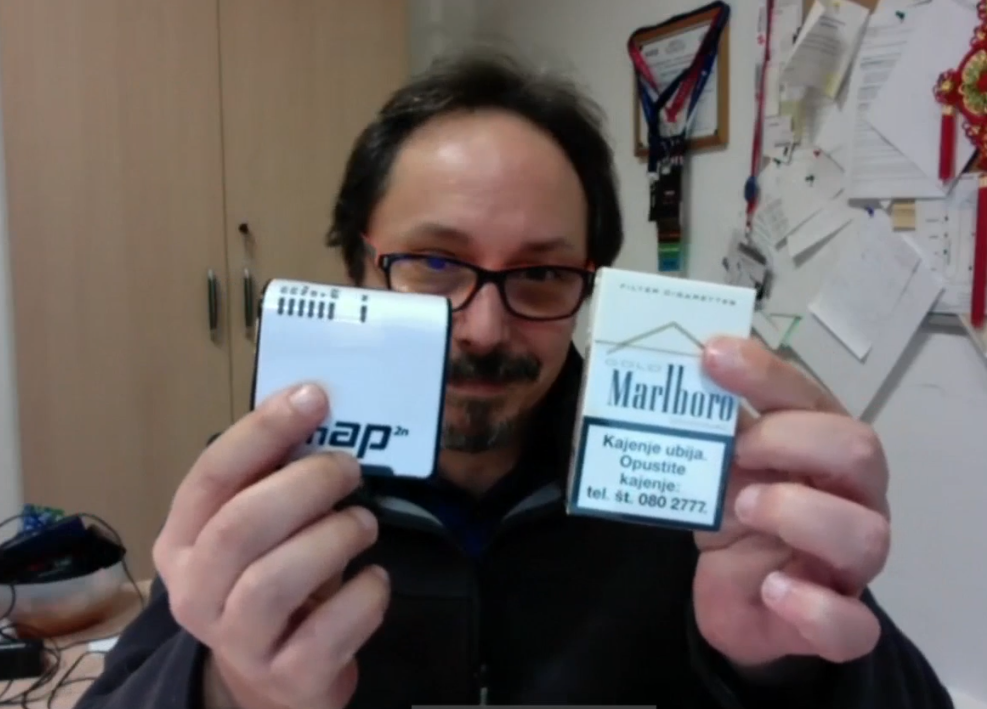
\includegraphics[scale=0.5]{img/fw_physical_cigarettes.png}
    \decoRule
    \caption{Prof. Pecorella showing how small is a home firewall compared to a pack of cigarettes.}
    \label{fig:fw_physical_cigarettes}
\end{figure}

A real home firewall costs about \$100 and is not larger than a pack of cigarettes (fig. \ref{fig:fw_physical_cigarettes}\footnote{No advertisement intended; smoke is not good for your health. The prof. should quit, too, as we like him and do not want anything bad to happen to him.}). It cannot withstand too much traffic, so it should only be used at home or for a small business (SOHO\footnote{Small office, home office.}).

Keep in mind that the IPv4 conntrack is different from its IPv6 equivalent, and the two stacks are largely independent, so we must not forget to write the same rules for each of them. Currently, our own firewall probably contains no rules because it has not been configured: for IPv4 this means that there are no security measures, while in IPv6 it means that our home appliances have a public global address that is unfirewalled and open to the Internet, and anybody could speak to them directly from all over the world. So yes, you should at least try to configure your firewall like, right now. Remember that rules are applied in the order they are written, so swapping two lines does not yield the same result, and as a side effect it might also impact the efficiency of the firewall\footnote{Many higher-level configurators, like Shorewall, implement extra rules for better efficiency.}. Just do not copy-paste everything you find on the Internet, or else you might make things worse (be extra careful when inserting IP addresses of any kind).

In fact, a general suggestion is to \textbf{never use raw configurations} nor copy firewall configurations from somebody else. The first one because higher-level configurators will \textit{translate} our rules into low-level firewall rules, and for this reason they must be well-maintained and trusted programs, the other option being directly dabbling with the firewall rules - which, as has already been tirelessly stated, can be quite dangerous.

The second suggestion comes from the fact that it is far too simple to find people online who posted their fantastic ultra nice firewall configuration saying "it worked for me": in the best case it might not work for us, while in the worst it might have rules that could open wide doors to our system. If we really want to copy something, it must be the simplest, most barebone thing, and nonetheless we should carefully study it before pasting it.

Last but not least, \textit{also} remember that iptables is a sort of man-in-the-middle between the actual Netfilter application and the user (an interface); in order to avoid mistakes (or at least reduce them), it is better to use something like Shorewall, a higher-level configurator with a better, much clearer interface.

All in all, it is better to stay and feel unprotected rather than feeling partially protected but without knowing what we are being protected from. Firewalls mean more than other things that we need manuality: we have to take some time and \textit{really} understand what we are doing. Setting up \textbf{virtual machines} and placing firewalls between them is a good way to start dabbling with firewalls while making sure to not damage anything.

%----------------------

\subsubsection*{pfSense}
An example of firewall is pfSense. It is an open source firewall, based on the OpenBSD\footnote{OpenBSD is a security-focused, free and open-source, Unix-like operating system based on the Berkeley Software Distribution (BSD) which emphasizes "portability, standardization, correctness, proactive security and integrated cryptography".} packet filter tool, \textit{pf}.

Between iptables and pfSense, prof. Pecorella highly suggests pfSense, because it comes out of the box with full support for redundancy, state replication and clustering. What we saw for Linux' iptables, however, does not apply to pfSense: the general idea is the same, but we would have to re-learn it.